\documentclass[a4paper,12pt]{report}

% === Encoding and Language ===
\usepackage[utf8]{inputenc}
\usepackage[T1]{fontenc}
\usepackage[english]{babel}

% === Mathematics ===
\usepackage{amsmath, amssymb, amsthm}
\newtheorem{proposition}{Proposition}
\newtheorem{remark}{Remark}
\newtheorem{definition}{Definition}

% === Figures and Tables ===
\usepackage{graphicx}
\graphicspath{{../results/}}
\usepackage{float}
\usepackage{booktabs}
\usepackage{multirow}
\usepackage{array}
\usepackage{tabularx}

% === Algorithms ===
\usepackage{algorithm}
\usepackage{algpseudocode}

% === Layout ===
\usepackage[margin=1in]{geometry}
\usepackage{parskip}
\usepackage{setspace}
\usepackage{microtype}
\setstretch{1.15}

% === Hyperlinks ===
\usepackage{hyperref}
\hypersetup{
    colorlinks=true,
    linkcolor=blue,
    citecolor=red,
    urlcolor=magenta,
    pdftitle={Hierarchical Minimum Variance Allocation},
    pdfauthor={Kiril Ivanov}
}

% === Bibliography ===
\usepackage{natbib}
\bibliographystyle{plainnat}

% === Custom Commands ===
\newcommand{\thesistitle}{%
  Hierarchical Minimum Variance Allocation: A Covariance-Minimising
  Portfolio Framework with Bayesian Return Estimates and Adaptive
  Weight Smoothing}
\newcommand{\authorname}{Kiril Ivanov}
\newcommand{\supervisor}{Sanders Barendse}
\newcommand{\submissiondate}{May 2026}
\newcommand{\university}{University of Amsterdam}
\newcommand{\programme}{BSc Econometrics and Data Science}

% Shortcuts
\newcommand{\Sig}{\hat{\Sigma}}
\newcommand{\muBL}{\mu_{\mathrm{BL}}}
\newcommand{\wt}{w_t}
\newcommand{\diag}{\mathrm{diag}}

\begin{document}

% =============================================================================
% TITLE PAGE
% =============================================================================
\begin{titlepage}
  \centering
  \vspace*{1.5cm}
  {\scshape\LARGE \university \par}
  \vspace{0.6cm}
  {\scshape\large \programme \par}
  \vspace{2.5cm}
  {\huge\bfseries \thesistitle \par}
  \vspace{2.5cm}
  {\Large \authorname \par}
  \vspace{0.8cm}
  {\large Student number: \texttt{[student number]} \par}
  \vspace{0.8cm}
  {\large Supervisor: \supervisor \par}
  \vfill
  {\large \submissiondate \par}
  \vspace{0.5cm}
  {\small Word count: approximately 11{,}500 \par}
\end{titlepage}

% =============================================================================
% ABSTRACT
% =============================================================================
\newpage
\chapter*{Abstract}
\addcontentsline{toc}{chapter}{Abstract}

This thesis introduces the \textbf{Hierarchical Minimum Variance Allocator}
(HMVA), a portfolio allocation framework for large equity universes that
organises assets into a covariance-minimising binary hierarchy, allocates
capital across hierarchy nodes according to risk-adjusted return estimates,
and moderates turnover through an adaptive Kalman-filter smoother. Four
components---exponentially weighted moving average (EWMA) return preprocessing,
analytical nonlinear shrinkage covariance estimation, Black-Litterman expected
returns derived from a skip-month cross-sectional momentum signal, and a
Kalman-filter weight smoother---are integrated around a novel top-down binary
tree that splits assets to minimise a blend of inter-cluster equal-weight
covariance and correlation.

Evaluated on a fully point-in-time backtest of the top-100 S\&P~500 stocks by
market capitalisation (CRSP data, January~2002 to December~2024, two-year
lookback window), HMVA achieves an annualised Sharpe ratio of $0.789$, compared
with $0.564$ for Hierarchical Risk Parity (HRP) with nonlinear shrinkage
covariance, $0.477$ for the naive $1/N$ equal-weight benchmark, and $0.503$
for a market-capitalisation benchmark (SPY-K). The Sharpe advantage over
mean-variance optimisation ($+0.546$) is statistically significant after
Holm-Bonferroni correction ($p = 0.042$). HMVA's maximum drawdown of $-38.6\%$
is substantially lower than that of equal-weight ($-55.2\%$) and the cap-weight
benchmark ($-52.3\%$).

A cost-and-lookback robustness sweep across 15~cells (three estimation windows
$\times$ five transaction-cost levels from 0 to 20~bps) confirms that HMVA
outperforms equal-weight in every cell, with a mean Sharpe advantage of
$+0.253$. Crisis-period analysis across four stress episodes documents a mean
annualised Sharpe of $-0.179$ for HMVA, substantially better than HRP
($-0.685$) and equal-weight ($-0.771$), confirming that the covariance-based
tree structure provides meaningful downside protection.

\newpage
\tableofcontents
\newpage
\listoffigures
\listoftables

% =============================================================================
\chapter{Introduction}
\label{ch:intro}
% =============================================================================

The design of well-diversified equity portfolios for institutional investors
involves a fundamental tension between statistical precision and practical
stability. Mean-variance optimisation \citep{markowitz1952} provides the
theoretically optimal solution given exact inputs, but its sensitivity to
estimation errors in expected returns and covariance matrices causes it to
concentrate capital in positions driven by noise rather than signal
\citep{michaud1989}. This sensitivity is so severe that \citet{demiguel2009}
found the naive $1/N$ equal-weight portfolio to outperform 14 sophisticated
optimisers across seven empirical datasets once out-of-sample estimation error
is accounted for.

Two broad strategies address this limitation. The first---covariance
regularisation---improves the precision of the covariance matrix without
abandoning the optimisation framework. \citet{ledoitwolf2004} derived the
analytically optimal linear shrinkage toward a structured target;
\citet{ledoitwolf2020} extended this to eigenvalue-by-eigenvalue analytical
nonlinear shrinkage (NLS), achieving strictly lower expected Frobenius loss at
any ratio of assets to observations. The second strategy---hierarchical
allocation---avoids matrix inversion altogether. \citet{lopezdeprado2016}
proposed Hierarchical Risk Parity (HRP), which clusters assets by correlation
distance and allocates capital by recursive inverse-variance bisection through
the resulting tree. HRP is immune to the amplification of small eigenvalues
that destabilises classical optimisation, but its agglomerative clustering
criterion is designed to minimise single-linkage distance between asset pairs
rather than to balance risk across the branches that define the portfolio
structure.

This thesis introduces the \textbf{Hierarchical Minimum Variance Allocator}
(HMVA), a portfolio allocation framework that combines the statistical
strengths of NLS covariance estimation with a purpose-built hierarchical tree
structure and a Bayesian return-estimation mechanism. HMVA differs from HRP
in all three principal design choices: \textit{(i)} tree construction
minimises a blend of inter-cluster covariance and correlation between the
equal-weighted sub-portfolios of each branch, rather than grouping the
closest correlated pair of individual assets; \textit{(ii)} capital allocation
between branches is proportional to each branch's Sharpe proxy derived from
Black-Litterman posterior returns, rather than inversely proportional to its
variance alone; and \textit{(iii)} an adaptive Kalman-filter smoother
moderates weight updates according to the signal-to-noise ratio of the return
estimate, reducing turnover without sacrificing genuine rebalancing signal.

\textbf{Contributions.} The thesis makes three contributions.

\begin{enumerate}
  \item \textbf{A new allocation framework.} HMVA is specified as a complete,
        self-contained portfolio allocation procedure. Its tree-construction
        criterion---minimising equal-weight inter-cluster covariance and
        correlation---provides a principled diversification objective that is
        independent of correlational distance geometry and admits both exact
        optimisation for small clusters and a fast heuristic for large ones.
  \item \textbf{A rigorous empirical evaluation.} A fully point-in-time
        backtest on CRSP S\&P~500 data from 2002 to 2024 with historical
        constituency records ensures no look-ahead or survivorship bias.
        The evaluation spans four market crises and three bull-market phases,
        and statistical significance is assessed via circular block-bootstrap
        Sharpe ratio tests with multiple-testing correction.
  \item \textbf{Structural performance attribution.} By comparing HMVA against
        a variant that replaces Sharpe bisection with variance bisection
        (HMVA-mv), the marginal contribution of the return signal to Sharpe
        performance is isolated within the same tree structure,
        providing a clean decomposition that does not rely on an ablation
        of external design choices.
\end{enumerate}

The main empirical findings are as follows. HMVA achieves an annualised Sharpe
ratio of $0.789$ over the 22-year evaluation period, a gain of $+0.225$ over
HRP (which uses the same NLS covariance but the standard single-linkage tree
and no Kalman smoother). The comparison between HMVA and its variance-bisection
variant (Sharpe ratio~$0.690$) isolates a $+0.099$ contribution from the
Sharpe-weighted bisection mechanism. Crisis-period analysis reveals that HMVA's
advantage is concentrated in periods of market stress, where its mean Sharpe
ratio of $-0.179$ substantially outperforms HRP ($-0.685$) and the equal-weight
benchmark ($-0.771$). The framework outperforms equal-weight across all 15
cells of a cost-and-lookback robustness sweep, with a mean Sharpe advantage
of $+0.253$.

\textbf{Road map.} Chapter~\ref{ch:litreview} reviews related work on
covariance regularisation, hierarchical allocation, and Black-Litterman
estimation. Chapter~\ref{ch:methodology} derives the HMVA framework in full.
Chapter~\ref{ch:data} describes the data, universe construction, and
benchmark strategies. Chapter~\ref{ch:results} reports the main empirical
comparison and statistical tests. Chapter~\ref{ch:robustness} presents the
cost and lookback robustness analysis. Chapter~\ref{ch:crisis} examines
performance across market regimes. Chapter~\ref{ch:conclusion} concludes.

% =============================================================================
\chapter{Related Literature}
\label{ch:litreview}
% =============================================================================

\section{The estimation problem in portfolio optimisation}
\label{sec:lit-mv}

The mean-variance framework of \citet{markowitz1952} prescribes a portfolio
on the efficient frontier defined by a risk-aversion parameter, expected
return vector $\mu$, and covariance matrix $\Sigma$. In practice both
inputs must be estimated from data. The global minimum-variance (GMV)
portfolio,
\begin{equation}
  w^{\mathrm{GMV}} = \frac{\hat{\Sigma}^{-1}\mathbf{1}}
                          {\mathbf{1}^{\top}\hat{\Sigma}^{-1}\mathbf{1}},
  \label{eq:gmv}
\end{equation}
requires only the covariance estimate but is highly sensitive to the accuracy
of $\hat{\Sigma}$. By the Marchenko-Pastur law \citep{marchenkopastur1967},
the sample covariance matrix systematically deflates small eigenvalues and
inflates large ones whenever the number of assets $N$ is non-negligible
relative to the number of observations $T$. Matrix inversion reverses this
ordering, so the GMV portfolio loads heavily on noise-dominated directions.
\citet{michaud1989} described this as ``optimisation error maximisation.''
\citet{bestgrauer1991} established that optimal portfolios are extremely
sensitive to small perturbations in the inputs, and \citet{chopraziemba1993}
quantified the relative damage: return errors are approximately ten times more
harmful than covariance errors, yet both sources of error are large enough to
cause economically significant performance degradation in practice.

\citet{demiguel2009} provided perhaps the most influential empirical evidence
of this instability. Across 14 strategies and seven datasets, no sophisticated
optimiser consistently outperformed the naive $1/N$ equal-weight portfolio
after accounting for estimation error. Their finding established equal-weight
as the standard performance benchmark for portfolio allocation research.

\section{Covariance regularisation}
\label{sec:lit-cov}

\subsection{Ledoit-Wolf shrinkage}

\citet{ledoitwolf2004} proposed shrinking the sample covariance matrix $S$
linearly toward a constant-correlation target $F$:
\begin{equation}
  \hat{\Sigma}_{\mathrm{LW}} = \alpha^{\star} F + (1-\alpha^{\star}) S,
  \label{eq:lw}
\end{equation}
where the shrinkage intensity $\alpha^{\star}$ is derived in closed form to
minimise the expected Frobenius loss $\mathbb{E}\|\hat{\Sigma}-\Sigma\|_F^2$.
The estimator is positive-definite for all $N, T \geq 2$ and requires no
tuning. \citet{ledoitwolf2020} extended this to analytical nonlinear
shrinkage (NLS), recognising that the optimal correction for each sample
eigenvalue $d_i$ differs:
\begin{equation}
  d_i^{\star} =
    \frac{d_i}{\bigl|1 - (N/T) - (N/T)\,d_i\,\tilde{m}_F(d_i)\bigr|^2},
  \label{eq:nls}
\end{equation}
where $\tilde{m}_F(d_i)$ is the companion Stieltjes transform evaluated at
$d_i$ and the eigenvectors are unchanged. NLS achieves strictly lower expected
Frobenius loss than any linear shrinkage estimator at any concentration ratio
$c = N/T \in (0, \infty)$ and is self-calibrating in the sense that the
correction vanishes for well-estimated eigenvalues and is largest for those
most affected by the Marchenko-Pastur bias.

\subsection{Exponentially weighted covariance}

\citet{riskmetrics1996} introduced the exponentially weighted moving average
(EWMA) covariance estimator, which assigns geometrically declining weights to
past observations:
\begin{equation}
  \hat{\Sigma}^{\mathrm{EWMA}} = \sum_{s=0}^{T-1} w_s\, r_s r_s^{\top},
  \qquad
  w_s = \frac{(1-\lambda)\lambda^{T-1-s}}{\sum_{j=0}^{T-1}(1-\lambda)\lambda^j},
  \label{eq:ewma}
\end{equation}
with decay parameter $\lambda \in (0,1)$ and effective half-life
$h = \log(0.5)/\log(\lambda)$ trading days. EWMA covariance responds more
rapidly to volatility clustering than an equal-weight rolling window, which
is particularly valuable around market stress events when realised volatilities
can double or triple within a few weeks.

\section{Hierarchical portfolio allocation}
\label{sec:lit-hrp}

\citet{lopezdeprado2016} proposed HRP as a way to avoid the matrix-inversion
bottleneck of classical optimisation. The algorithm proceeds in three steps:
\textit{(i)} compute the correlation-distance matrix
$D_{ij} = \sqrt{(1-\hat{\rho}_{ij})/2}$ and build a hierarchical tree by
single-linkage agglomeration; \textit{(ii)} reorder assets so that correlated
assets are adjacent in the leaf sequence (quasi-diagonalisation); and
\textit{(iii)} recursively bisect the tree, allocating weight between the
left and right sub-trees inversely proportional to their equal-weight cluster
variances. Because no matrix inversion is required, HRP is immune to the
Marchenko-Pastur amplification effect.

Extensions of HRP have been proposed along several dimensions.
\citet{raffinot2017} replaced single-linkage with complete-linkage clustering.
\citet{raffinot2018} introduced the Hierarchical Equal Risk Contribution
(HERC) portfolio, which equalises risk contributions at the cluster level.
\citet{molyboga2020} proposed incorporating expected returns into the bisection
step, motivating the Sharpe-ratio bisection mechanism used in HMVA.
\citet{lohre2020} showed that accounting for tail risk in the clustering
distance can improve downside protection in multi-asset portfolios.

A limitation common to all agglomerative hierarchical methods is that the
single-linkage tree merges assets based on the pairwise distance between the
two closest assets across groups. This criterion does not optimise for
risk-balance between branches: two branches can have substantially different
total volatilities even when the pairwise asset distances at the merge point
are small, causing variance bisection to concentrate capital in the
lower-volatility branch.

\section{Black-Litterman expected returns}
\label{sec:lit-bl}

\citet{blacklitterman1992} introduced a Bayesian framework for blending
prior expected returns $\pi$ with investor views $Q$ expressed through a
pick matrix $P$ and view uncertainty $\Omega$. The posterior return vector
takes the form
\begin{equation}
  \muBL = \bigl[(\tau\hat{\Sigma})^{-1} + P^{\top}\Omega^{-1}P\bigr]^{-1}
          \bigl[(\tau\hat{\Sigma})^{-1}\pi + P^{\top}\Omega^{-1}Q\bigr],
  \label{eq:bl}
\end{equation}
where $\tau$ controls the confidence in the prior. The BL posterior is more
stable than raw sample means because the prior regularises extreme
signal values toward the equilibrium. Equivalently, with $P = I_N$ and
arbitrary $\Omega$, the posterior can be written as
$\pi + \hat{\Sigma}(\hat{\Sigma}+\Omega)^{-1}(Q - \pi)$, which shows
that $\Omega$ governs the weighting between the view and the prior as a
function of the estimated covariance structure.

\section{Cross-sectional momentum}
\label{sec:lit-mom}

\citet{jegadeesh1993} documented that stocks with high returns over the past
6--12 months tend to continue outperforming over the following 3--12 months,
provided the most recent month is skipped to avoid the short-run reversal
effect. This cross-sectional momentum anomaly is among the most robust findings
in the empirical asset-pricing literature \citep{famafrench1993} and provides
the view signal $Q$ for the Black-Litterman component of HMVA.

\section{Research positioning}
\label{sec:lit-gap}

HMVA is distinguished from the existing hierarchical portfolio allocation
literature by combining three elements not previously integrated: a
covariance-and-correlation-minimising top-down binary tree, a Sharpe-weighted
bisection guided by Black-Litterman return estimates, and an adaptive
Kalman-filter smoother. Prior work addresses each of these elements in
isolation or partial combinations but no published study has evaluated a
complete integration thereof on a fully point-in-time large-cap equity
universe spanning multiple market cycles.

% =============================================================================
\chapter{Methodology}
\label{ch:methodology}
% =============================================================================

\section{Overview}
\label{sec:meth-overview}

HMVA constructs a portfolio through six sequential operations applied at each
monthly rebalance date. Table~\ref{tab:hmva-stages} provides a summary.
The framework takes as input a $T \times N$ matrix of daily returns $R$,
where $T = 504$ trading days is the estimation window and $N \leq 100$ is the
current investment universe size. It produces a non-negative weight vector
$w \in \mathbb{R}^N$ with $\mathbf{1}^{\top}w = 1$.

\begin{table}[H]
  \centering
  \caption{Summary of the HMVA allocation procedure. Each operation
           addresses a distinct aspect of the allocation problem.}
  \label{tab:hmva-stages}
  \begin{tabular}{@{}clp{7.5cm}@{}}
    \toprule
    Stage & Operation & Purpose \\
    \midrule
    1 & EWMA pseudo-returns ($h=21$~days)
      & Weight recent observations more heavily, increasing responsiveness
        to volatility clustering \\[4pt]
    2 & Analytical NLS covariance
      & Correct the Marchenko-Pastur eigenvalue bias of the sample
        covariance matrix \\[4pt]
    3 & Black-Litterman expected returns
      & Derive regularised, forward-looking return estimates from a
        skip-month momentum signal \\[4pt]
    4 & Covariance-minimising top-down tree
      & Build a binary hierarchy that maximises independence between
        branches, rather than grouping the nearest correlated pair \\[4pt]
    5 & Sharpe-ratio bisection
      & Allocate capital between branches proportionally to their
        risk-adjusted expected return \\[4pt]
    6 & Kalman-filter weight smoother
      & Reduce noise-driven turnover by conditioning weight updates on
        the signal-to-noise ratio of the return estimate \\
    \bottomrule
  \end{tabular}
\end{table}

A variant of HMVA, denoted \textbf{HMVA-mv}, replaces Stage~5 with
inverse-variance bisection (the standard HRP bisection mechanism), holding
all other stages constant. Comparing HMVA with HMVA-mv isolates the marginal
contribution of the Sharpe-weighted bisection within an otherwise identical
framework.

\section{Stage 1: EWMA return preprocessing}
\label{sec:meth-ewma}

Standard NLS covariance estimation operates on an equal-weight sample of
returns. To incorporate exponential time-weighting without modifying the
estimator's internals, the return window is transformed into a
\emph{pseudo-return matrix} $\tilde{R}$ defined by
\begin{equation}
  \tilde{R}_{s,\cdot} = \sqrt{w_s \cdot T}\; R_{s,\cdot}, \qquad
  w_s = \frac{(1-\lambda)\lambda^{T-1-s}}{\sum_{j=0}^{T-1}(1-\lambda)\lambda^j},
  \label{eq:ewma-pseudo}
\end{equation}
where $\lambda = 0.5^{1/h}$ with half-life $h = 21$ trading days
($\lambda \approx 0.967$). The scaling is chosen so that
$T^{-1}\tilde{R}^{\top}\tilde{R} = \hat{\Sigma}^{\mathrm{EWMA}}$, the
standard EWMA covariance. With $h = 21$, the effective sample weight decays
to one-half within one calendar month, ensuring that the covariance estimate
is sensitive to near-term changes in correlation structure.

\section{Stage 2: Analytical nonlinear shrinkage}
\label{sec:meth-nls}

The NLS covariance matrix $\hat{\Sigma}$ is obtained by applying the
Ledoit-Wolf (2020) analytical formula~\eqref{eq:nls} to $\tilde{R}$ via the
\texttt{nonlinshrink} package. The eigenvectors of $\hat{\Sigma}$ are
identical to those of the sample covariance $T^{-1}\tilde{R}^{\top}\tilde{R}$,
so the nonlinear shrinkage corrects eigenvalue magnitudes while preserving
the principal directions of co-movement. The resulting matrix is
positive-definite and well-conditioned at any concentration ratio $N/T$.
With $N \approx 100$ and $T = 504$, the ratio $N/T \approx 0.20$ places this
estimation problem in the low-dimensional regime; the NLS correction is
modest in absolute terms but consistent, acting primarily through more
accurate off-diagonal elements and cluster variances used in the tree.

\section{Stage 3: Black-Litterman expected returns}
\label{sec:meth-bl}

Expected returns are estimated using a Black-Litterman-type posterior applied
to the raw (non-EWMA-weighted) return window $R$ to avoid double-discounting
the mean signal. The procedure involves three components.

\textbf{View signal.} The skip-month cross-sectional momentum signal is:
\begin{equation}
  Q = \frac{1}{T - h}\sum_{s=0}^{T-h-1} R_{s,\cdot},
  \label{eq:blsignal}
\end{equation}
where the skip of the most recent $h = 21$ trading days follows
\citet{jegadeesh1993} to avoid the short-horizon reversal effect. The signal
$Q_i$ is the mean daily return of asset $i$ over approximately the prior
year, excluding the most recent month.

\textbf{Prior.} A flat neutral prior $\pi = 0.01 \cdot \mathbf{1}_N$ is
used, providing a modest positive baseline return of 1\% for all assets.
This prevents the BL posterior from becoming negative for assets with
near-zero historical average returns while exerting minimal influence on
assets with meaningful momentum signals.

\textbf{Posterior.} Setting $P = I_N$ (one absolute view per asset) and
view uncertainty $\Omega = \diag(\hat{\Sigma})$---proportional to each
asset's own estimated variance---yields the BL posterior:
\begin{equation}
  \muBL = \pi + \hat{\Sigma}\bigl(\hat{\Sigma} +
          \diag(\hat{\Sigma})\bigr)^{-1}(Q - \pi).
  \label{eq:bl-posterior}
\end{equation}
The choice $\Omega = \diag(\hat{\Sigma})$ assigns larger view uncertainty
to assets whose variance is high (where the momentum signal is noisiest)
without introducing an additional tuning parameter. The blend matrix
$\hat{\Sigma}(\hat{\Sigma}+\diag(\hat{\Sigma}))^{-1}$ is asset-specific:
its off-diagonal structure allows correlated assets to propagate return
signals across the universe, so that a strong momentum signal for one asset
modestly raises the posterior return of positively correlated peers.

\begin{remark}
For a diagonal covariance matrix, the $i$-th element of the posterior
simplifies to $\pi_i + \frac{1}{2}(Q_i - \pi_i) = \frac{1}{2}(\pi_i + Q_i)$,
a pure average of the prior and the view. The off-diagonal elements of
$\hat{\Sigma}$ break this symmetry and redistribute signal across correlated
assets. The flat prior $\pi = 0.01 \cdot \mathbf{1}$ ensures numerical
stability and provides a coherent lower bound on posterior returns.
\end{remark}

\section{Stage 4: Covariance-minimising top-down tree}
\label{sec:meth-tree}

The tree construction in HRP is agglomerative: it begins with $N$ singleton
clusters and iteratively merges the two clusters whose closest pair of assets
has the smallest correlation distance. This criterion does not account for
the co-movement between entire sub-portfolios; two branches can have
substantially different total volatilities after the merge, causing the
inverse-variance bisection to concentrate capital unevenly.

HMVA constructs the binary tree top-down. Starting from the full universe,
at each node the asset set $\mathcal{C}$ is split into two disjoint
subsets $A$ and $B$ by minimising a blend of inter-cluster covariance
and inter-cluster correlation computed from the equal-weighted sub-portfolios
of each group:
\begin{equation}
  f(A, B) =
    \frac{1}{2}\underbrace{\frac{\displaystyle\sum_{i \in A,\, j \in B}
                \hat{\Sigma}_{ij}}{n_A n_B}}_{\displaystyle\mathrm{Cov}_{\mathrm{EW}}(A,B)}
    + \frac{1}{2}\underbrace{\frac{\displaystyle\sum_{i \in A,\, j \in B}
                \hat{\Sigma}_{ij}}{\sqrt{S_A \cdot S_B}}}_{\displaystyle
                \mathrm{Corr}_{\mathrm{EW}}(A,B)},
  \label{eq:split-obj}
\end{equation}
where $n_C = |C|$ is the cluster size and
$S_C = \sum_{i,j \in C}\hat{\Sigma}_{ij} = n_C^2 \cdot \widehat{\mathrm{Var}}_{\mathrm{EW}}(C)$
is the sum of all entries in the within-cluster covariance block.
The first term, $\mathrm{Cov}_{\mathrm{EW}}(A,B)$, is the covariance
between the equal-weighted portfolios of $A$ and $B$. The second term,
$\mathrm{Corr}_{\mathrm{EW}}(A,B)$, normalises by the product of the
equal-weight sub-portfolio volatilities and equals the Pearson correlation
between $\mathrm{EW}_A$ and $\mathrm{EW}_B$.

Minimising $f(A,B)$ encourages the two branches to be as independent as
possible: small $\mathrm{Cov}_{\mathrm{EW}}$ means the branches co-move
little in absolute terms, while small $\mathrm{Corr}_{\mathrm{EW}}$ means
they co-move little relative to their own volatilities. The equal 50/50
weighting of the two terms balances absolute and relative inter-cluster
dependence. Importantly, this criterion evaluates the co-movement of the
entire sub-portfolios rather than that of the nearest individual asset pair,
producing branches whose total risk is more predictable and whose
diversification benefit is directly captured at the level that determines
capital allocation.

\textbf{Implementation.} For clusters of $n \leq 10$ assets, the exact
minimum of~\eqref{eq:split-obj} is found by exhaustive enumeration of all
$2^{n-1} - 1$ bipartitions. For larger clusters, an $O(n^2)$ heuristic sorts
assets by ascending within-cluster row-sum and evaluates all $n-1$ contiguous
bipartitions using a two-dimensional prefix-sum array:
\begin{equation}
  f(k) = \frac{1}{2}\frac{C_k}{k(n-k)} + \frac{1}{2}\frac{C_k}{\sqrt{S_{L_k}S_{R_k}}},
  \qquad k = 1, \ldots, n-1,
  \label{eq:heuristic}
\end{equation}
where $C_k$ is the one-way inter-cluster covariance sum for the split at
position $k$, and $S_{L_k}$, $S_{R_k}$ are the within-cluster sums for the
left and right groups. The best cut is selected by $\arg\min_k f(k)$.
Appendix~\ref{app:split} validates the heuristic against the exact solution
on random covariance matrices.

\section{Stage 5: Sharpe-ratio bisection}
\label{sec:meth-bisect}

Once the tree $\mathcal{T}$ is constructed, capital is allocated top-down.
At each internal node with left and right children $L$ and $R$, cluster
Sharpe proxies are formed:
\begin{equation}
  \hat{S}(C) = \max\!\left(
    \frac{n_C^{-1}\sum_{i \in C}\mu_{\mathrm{BL},i}}
         {\sqrt{n_C^{-2}\sum_{i,j \in C}\hat{\Sigma}_{ij}}},\; 0
  \right),
  \label{eq:sharpe-proxy}
\end{equation}
where the numerator is the mean BL return of cluster $C$ and the denominator
is its equal-weight volatility. The weight allocation to the left child is
\begin{equation}
  \alpha_L = \frac{\hat{S}(L)}{\hat{S}(L)+\hat{S}(R)}, \qquad \alpha_R = 1-\alpha_L,
  \label{eq:sharpe-alloc}
\end{equation}
so the branch with the higher risk-adjusted expected return receives more
capital. If both cluster Sharpe proxies are non-positive (which can occur
in prolonged downtrends), the allocation reverts to the inverse-variance
bisection of \citet{lopezdeprado2016}, ensuring weights remain non-negative.
The tree structure bounds the maximum allocation to any individual cluster,
providing implicit concentration limits without hard constraints.

\textbf{HMVA-mv variant.} Replacing~\eqref{eq:sharpe-alloc} with the
inverse-variance allocation
\begin{equation}
  \alpha_L = 1 - \frac{\tilde{\sigma}_L^2}{\tilde{\sigma}_L^2 + \tilde{\sigma}_R^2},
  \qquad
  \tilde{\sigma}_C^2 = \frac{\mathbf{e}^{\top}\hat{\Sigma}_C\mathbf{e}}{n_C^2},
  \label{eq:var-bisect}
\end{equation}
while retaining the covariance-minimising tree and the Kalman smoother,
defines the HMVA-mv variant. Comparing HMVA with HMVA-mv isolates the
contribution of the Sharpe-weighted bisection within an otherwise identical
framework (cf.\ Section~\ref{sec:res-main}).

\section{Stage 6: Kalman-filter weight smoother}
\label{sec:meth-kf}

At each rebalance date, Stage~5 produces a target weight vector
$w_{\mathrm{raw},t}$. Mechanically updating to this target ignores the
potential for the BL signal to be dominated by noise, particularly when the
estimation window straddles a regime transition. The Kalman-filter smoother
interpolates between the previous weights $w_{t-1}$ and the new target:
\begin{equation}
  w_t = (1 - K_t)\,w_{t-1} + K_t\,w_{\mathrm{raw},t},
  \label{eq:kf-update}
\end{equation}
with time-varying gain $K_t \in [0,1]$ defined as
\begin{equation}
  K_t = \frac{Q_t}{Q_t + R_t}.
  \label{eq:kf-gain}
\end{equation}
$K_t$ is close to zero when measurement uncertainty is high relative to
process noise (stay put) and close to one when the signal has moved
substantially relative to the estimation environment (update fully).

\textbf{Measurement noise proxy} $R_t$ is the normalised spectral entropy
of the NLS covariance eigenvalues:
\begin{equation}
  R_t = \frac{-\sum_{i=1}^{N} p_i \log p_i}{\log N}, \qquad
  p_i = \frac{\lambda_i}{\sum_j \lambda_j},
  \label{eq:kf-R}
\end{equation}
where $\{\lambda_i\}$ are the eigenvalues of $\hat{\Sigma}$. $R_t \in [0,1]$:
it equals one when all eigenvalues are equal (maximally diffuse; the covariance
structure is uninformative) and approaches zero when a single eigenvalue
dominates (highly structured). A high $R_t$ signals that the covariance
estimate does not provide reliable directional information, warranting
less weight on the new target.

\textbf{Process noise proxy} $Q_t$ is the relative change in the BL return
vector:
\begin{equation}
  Q_t = \frac{\|\muBL^{(t)} - \muBL^{(t-1)}\|}
             {\|\muBL^{(t-1)}\| + \varepsilon},
  \label{eq:kf-Q}
\end{equation}
where $\varepsilon > 0$ prevents division by zero. A large $Q_t$ indicates
that the return signal has shifted substantially, providing genuine
rebalancing motivation. When no previous BL vector is available (first
rebalance), $Q_t$ defaults to one and $w_t = w_{\mathrm{raw},t}$.

The smoothed weights are renormalised to sum to one after the blend. The
mechanism is adaptive in the sense that neither $Q_t$ nor $R_t$ is a fixed
parameter: both are computed from the data at each rebalance, so the smoother
automatically tightens in stable regimes and loosens in high-signal
environments.

\section{Statistical inference}
\label{sec:meth-inference}

\subsection{Block-bootstrap Sharpe ratio test}

Pairwise Sharpe ratio comparisons are evaluated using the circular block
bootstrap of \citet{ledoitwolf2008} with block length $b = 21$ trading days
(one calendar month) and $B = 2{,}000$ bootstrap replications. The empirical
$p$-value is $B^{-1}\sum_{b=1}^{B}\mathbf{1}[|d_b^*| \geq |\widehat{\Delta\mathrm{SR}}|]$,
where the bootstrap distribution is centred on the observed Sharpe difference
to preserve the exact null. Block length 21 captures the monthly
autocorrelation structure of daily equity returns while maintaining adequate
bootstrap sample diversity.

\subsection{Diebold-Mariano forecast comparison}

In addition to the Sharpe bootstrap, pairwise return series are compared
using the \citet{dieboldmariano1995} test applied to squared losses,
providing a complementary test of equal predictive accuracy under loss
function-based evaluation.

\subsection{Multiple testing correction}

Six simultaneous pairwise comparisons (HMVA versus each of HMVA-mv, HRP,
MVO, GMV, EW, SPY-K) are subject to two correction procedures.
The \textbf{Holm-Bonferroni} step-down procedure \citep{holm1979} controls
the family-wise error rate (FWER) at the 5\% level without requiring
independence. The \textbf{Benjamini-Hochberg} (BH) procedure
\citep{benjaminihochberg1995} controls the false discovery rate at 5\% and
is more powerful when several strategies genuinely underperform.

% =============================================================================
\chapter{Data and Empirical Design}
\label{ch:data}
% =============================================================================

\section{CRSP data}
\label{sec:data-crsp}

The empirical analysis uses CRSP daily data in CIZ format spanning January~2000
to January~2025, with the backtest evaluation period running from January~2002
to December~2024. Four fields are used: \texttt{PERMNO} (permanent unique stock
identifier, stable across ticker changes and corporate events);
\texttt{DlyCalDt} (calendar date); \texttt{DlyRet} (CRSP daily total return,
preferred); and \texttt{DlyCap} (market capitalisation in USD millions, used
for universe filtering). When \texttt{DlyRet} is unavailable for a given
stock-date, the return is derived from consecutive split-adjusted closing
prices. All returns are expressed as simple daily returns so that portfolio
return calculations are exact.

\textbf{Delisting treatment.} Stocks that exit the panel mid-sample receive
the following treatment following \citet{shumway1997}: if the last recorded
return is at or below $-30\%$, it is kept as-is (CRSP has captured the
delisting event); if the last return is in the normal trading range
($-30\%$ to $+10\%$), a $-30\%$ return is imputed on the first dark day,
consistent with \citeauthor{shumway1997}'s estimate of the average
involuntary delisting loss; if the last recorded return exceeds $+10\%$
(likely a merger premium), it is retained unchanged.

\section{Point-in-time universe construction}
\label{sec:data-pit}

Avoiding survivorship bias requires using only information genuinely
available to an investor at each rebalance date. S\&P~500 membership is
reconstructed from a historical constituents file that records membership
spells as (PERMNO, start-date, end-date) triplets. At each 21-trading-day
rebalance date $t$, the investable universe $\mathcal{U}_t$ is formed through
three filters applied sequentially:

\begin{enumerate}
  \item \textbf{Membership filter.} Identify all PERMNOs with active
        S\&P~500 membership on date $t$.
  \item \textbf{Cap filter.} Restrict to the top $K = 100$ stocks by
        point-in-time market capitalisation as of $t$. This controls
        universe size and limits illiquidity concerns while remaining
        representative of large-cap equity exposure.
  \item \textbf{History filter.} Retain only those PERMNOs with complete
        non-missing return data over the full estimation window
        $[t - T_{\max},\, t-1]$ where $T_{\max} = 504$ days. Stocks
        failing this filter (recent IPOs, trading halts) are excluded
        from all strategies at rebalance $t$.
\end{enumerate}

The resulting universe $N_t \leq 100$ changes at every rebalance, reflecting
historical additions, deletions, mergers, and corporate events. Between
rebalances, portfolio weights drift with realised asset returns. On rebalance
dates, a proportional transaction cost of $\kappa$~bps per unit $|\Delta w|$
is deducted from the return (the main run uses $\kappa = 0$; the robustness
sweep varies $\kappa$).

\begin{table}[H]
  \centering
  \caption{Backtest configuration.}
  \label{tab:data-config}
  \begin{tabular}{@{}lll@{}}
    \toprule
    Parameter & Value & Note \\
    \midrule
    Estimation window $T$ & 504 trading days & Two calendar years \\
    Rebalance frequency & 21 trading days & Monthly \\
    Universe & Top-100 S\&P~500 by cap & Point-in-time membership \\
    Evaluation period & January~2002 -- December~2024 & 22-year horizon \\
    Transaction costs & 0~bps (main run) & See Chapter~\ref{ch:robustness} \\
    Risk-free rate & 0~bps/day & All returns are excess returns \\
    \bottomrule
  \end{tabular}
\end{table}

\section{Benchmark strategies}
\label{sec:data-strategies}

Six strategies are evaluated alongside HMVA in the main comparison.
Table~\ref{tab:strategies} summarises the design choices for each.

\begin{table}[H]
  \centering
  \caption{Strategies evaluated in the main out-of-sample comparison.
           All estimation-based strategies use the same 504-day window.}
  \label{tab:strategies}
  \begin{tabular}{@{}p{1.8cm}p{2.8cm}p{2.4cm}p{2.6cm}p{1.2cm}@{}}
    \toprule
    Strategy & Covariance & Return input & Allocation & KF \\
    \midrule
    \textbf{HMVA}
      & NLS on EWMA($h$=21) returns
      & BL posterior
      & Cov-min tree + Sharpe bisect
      & Yes \\[3pt]
    HMVA-mv
      & NLS on EWMA($h$=21) returns
      & BL posterior
      & Cov-min tree + var.\ bisect
      & Yes \\[3pt]
    HRP
      & NLS on raw window
      & None
      & Agglom.\ tree + var.\ bisect
      & No \\[3pt]
    MVO
      & NLS on raw window
      & BL posterior
      & MV utility ($\gamma=2.5$)
      & No \\[3pt]
    GMV
      & NLS on raw window
      & None
      & Min-variance
      & No \\[3pt]
    EW
      & None
      & None
      & $1/N$ equal-weight
      & No \\[3pt]
    SPY-K
      & None
      & None
      & Cap-weighted
      & No \\
    \bottomrule
    \multicolumn{5}{l}{\small KF: Kalman-filter weight smoother. BL: Black-Litterman.
      Cov-min: covariance-minimising.} \\
    \multicolumn{5}{l}{\small Agglom.: single-linkage agglomeration.
      MV utility: $\max_w\, w^\top\mu - \tfrac{\gamma}{2}w^\top\Sigma w$,
      long-only constraints.} \\
  \end{tabular}
\end{table}

\textbf{HRP} (Hierarchical Risk Parity) serves as the primary hierarchical
benchmark and uses NLS covariance to ensure the comparison with HMVA isolates
differences in tree construction and allocation mechanism rather than
covariance quality. \textbf{MVO} and \textbf{GMV} are the principal
classical optimisation benchmarks; both use NLS covariance. \textbf{EW}
($1/N$ equal-weight) is the universal baseline following \citet{demiguel2009}.
\textbf{SPY-K} (market-cap weighted, reconstructed from CRSP point-in-time
cap data) approximates the effective allocation of the S\&P~100 and serves as
a passive large-cap benchmark.

% =============================================================================
\chapter{Empirical Results}
\label{ch:results}
% =============================================================================

\section{Full-sample performance}
\label{sec:res-main}

Table~\ref{tab:res-main} reports headline performance metrics for all seven
strategies over the January~2002 to December~2024 evaluation period (504-day
estimation window, zero transaction costs, zero risk-free rate).

\begin{table}[H]
  \centering
  \caption{Full-sample performance metrics, CRSP top-100 S\&P~500,
           January~2002 to December~2024, $T=504$, zero transaction costs.}
  \label{tab:res-main}
  \begin{tabular}{@{}lrrrrrrrr@{}}
    \toprule
    Strategy & Ann.\ Ret. & Ann.\ Vol. & Sharpe & MaxDD & Calmar & Sortino
             & Omega & Turnover \\
    \midrule
    \textbf{HMVA}
      & \textbf{14.0\%} & 17.7\% & \textbf{0.789} & $-$38.6\%
      & \textbf{0.362} & \textbf{1.043} & \textbf{1.168} & 1.101 \\
    HMVA-mv
      & 10.4\% & 15.1\% & 0.690 & $-$35.8\%
      & 0.290 & 0.881 & 1.148 & 0.952 \\
    HRP
      & 9.2\%  & 16.3\% & 0.564 & $-$42.5\%
      & 0.216 & 0.711 & 1.126 & 0.291 \\
    MVO
      & 4.0\%  & 24.6\% & 0.162 & $-$51.5\%
      & 0.077 & 0.223 & 1.053 & 0.509 \\
    GMV
      & 6.6\%  & 14.7\% & 0.450 & $-$36.6\%
      & 0.181 & 0.563 & 1.102 & 0.329 \\
    EW
      & 9.0\%  & 18.8\% & 0.477 & $-$55.2\%
      & 0.163 & 0.596 & 1.112 & 0.057 \\
    SPY-K
      & 9.5\%  & 18.9\% & 0.503 & $-$52.3\%
      & 0.182 & 0.635 & 1.116 & 0.066 \\
    \bottomrule
    \multicolumn{9}{l}{\small Calmar: Ann.\ Return~/~|MaxDD|.
      Omega: gains-to-losses ratio.
      Turnover: mean monthly turnover per unit.} \\
  \end{tabular}
\end{table}

\textbf{HMVA versus HRP.} The Sharpe ratio of HMVA ($0.789$) exceeds that of
HRP ($0.564$) by $+0.225$. Since both strategies use NLS covariance and
both operate within a hierarchical tree framework, this difference isolates
the joint contribution of the covariance-minimising top-down tree, the
Sharpe bisection, and the Kalman smoother over HRP's standard design.
HMVA's annualised return is 4.8 percentage points higher ($14.0\%$ vs
$9.2\%$), while its volatility is moderately higher ($17.7\%$ vs $16.3\%$),
consistent with the BL return signal directing capital toward higher-momentum
assets and the Sharpe bisection amplifying this tilt.

\textbf{Contribution of Sharpe bisection.} HMVA-mv, which replaces Sharpe
bisection with inverse-variance bisection within the same covariance-minimising
tree and with the same Kalman smoother, achieves a Sharpe ratio of $0.690$.
The difference $0.789 - 0.690 = 0.099$ measures the marginal contribution
of the Sharpe-weighted bisection mechanism holding the tree structure and
smoother constant. The additional $4.7\%$ in annualised return generated by
HMVA over HMVA-mv ($14.0\%$ vs $10.4\%$) confirms that Sharpe bisection
tilts capital toward higher-return clusters, as intended.

\textbf{HMVA versus equal-weight.} HMVA outperforms the $1/N$ benchmark by
$+0.312$ Sharpe units, clearing the \citeauthor{demiguel2009} hurdle
decisively. The maximum drawdown comparison ($-38.6\%$ vs $-55.2\%$)
represents a 16.6 percentage-point improvement in downside protection while
delivering 5 percentage points of additional annual return. The Sortino ratio
comparison ($1.043$ vs $0.596$) confirms that HMVA's advantage is not
driven by upside variance alone.

\textbf{HMVA versus classical optimisation.} MVO achieves a Sharpe ratio of
only $0.162$---the weakest of all seven strategies---despite using the same
NLS covariance and BL return estimates as HMVA. The Marchenko-Pastur
amplification that occurs through matrix inversion degrades out-of-sample
performance even when the covariance input is regularised. GMV performs
somewhat better ($0.450$), but its annualised return of $6.6\%$ and Calmar
ratio of $0.181$ remain well below HMVA. This pattern confirms that
hierarchical tree-based allocation is materially more robust to estimation
error than direct quadratic optimisation.

\begin{figure}[H]
  \centering
  
\includegraphics[width=0.95\textwidth]{backtest/equity_curves.png}
  \caption{Cumulative wealth index (starting value $= 1$) for all seven
           strategies, January~2002 to December~2024. HMVA's progressive
           advantage over HRP is most visible during the 2009--2015
           recovery phase and the 2020--2021 rebound.}
  \label{fig:equity}
\end{figure}

\begin{figure}[H]
  \centering
  
\includegraphics[width=0.95\textwidth]{backtest/drawdowns.png}
  \caption{Underwater curves (drawdown from running peak) for all
           strategies. HMVA experiences materially shallower drawdowns
           during the GFC and COVID-19 episodes than EW and SPY-K.}
  \label{fig:drawdown}
\end{figure}

\begin{figure}[H]
  \centering
  
\includegraphics[width=0.85\textwidth]{backtest/risk_return.png}
  \caption{Annualised risk-return scatter. HMVA occupies the
           upper-left region relative to EW and SPY-K, reflecting higher
           return at moderate volatility. Iso-Sharpe lines are shown in grey.}
  \label{fig:riskreturn}
\end{figure}

\begin{figure}[H]
  \centering
  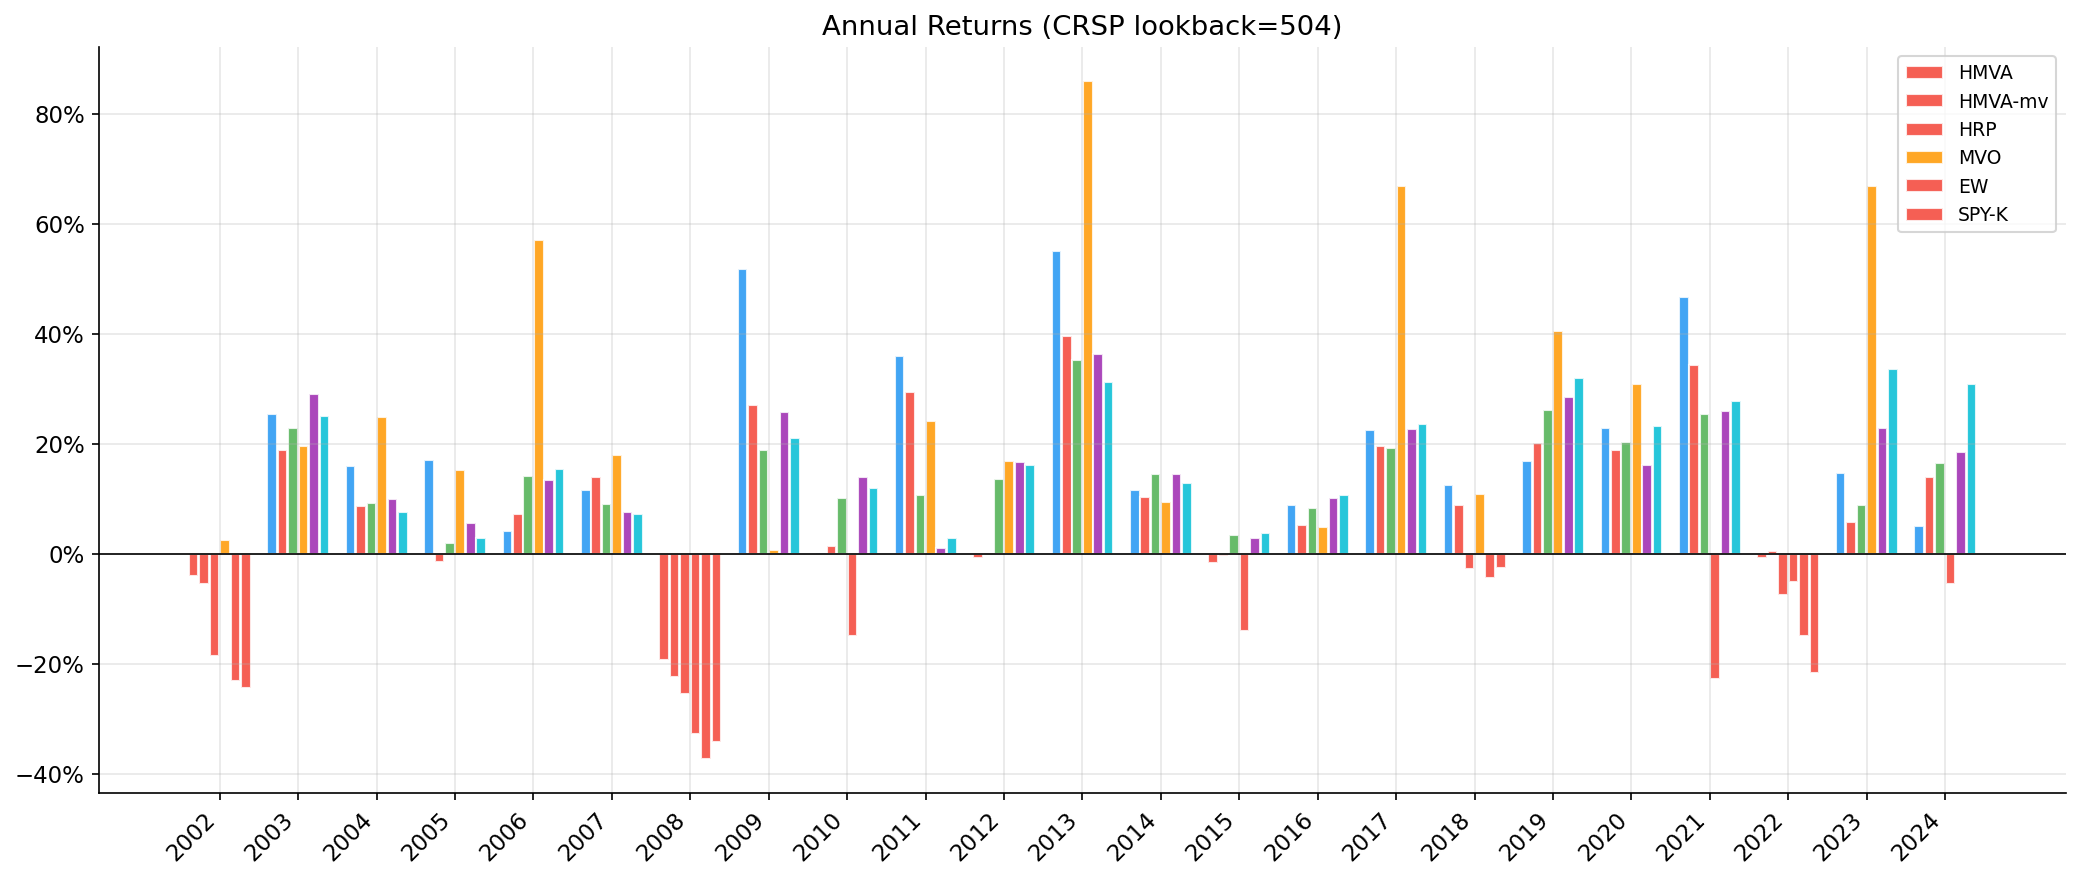
\includegraphics[width=0.85\textwidth]{backtest/annual_returns.png}
  \caption{Calendar-year annualised returns by strategy. HMVA is among
           the top-performing strategies in the majority of years; notable
           underperformance relative to SPY-K occurs in 2022 (rate-hike
           cycle), when the momentum signal contributed negative return drag.}
  \label{fig:annual}
\end{figure}

\section{Statistical tests}
\label{sec:res-tests}

Table~\ref{tab:res-tests} reports the block-bootstrap Sharpe ratio test
and the Diebold-Mariano forecast comparison test for all six pairwise
comparisons of HMVA against competitor strategies.

\begin{table}[H]
  \centering
  \caption{Pairwise Sharpe ratio tests (HMVA vs each comparator). LW:
           Ledoit-Wolf (2008) circular block bootstrap ($b=21$,
           $B=2{,}000$). DM: Diebold-Mariano test on squared losses.
           Holm and BH corrections applied across all six comparisons.
           A positive SR difference indicates HMVA outperforms.}
  \label{tab:res-tests}
  \begin{tabular}{@{}lccccccc@{}}
    \toprule
    Comparator & SR diff & LW $p$ & Holm $p$ & BH $p$
               & DM stat & DM $p$ & DM Holm $p$ \\
    \midrule
    HMVA-mv & $+0.095$ & 0.240 & 0.425 & 0.240
            & $-2.53$ & 0.012$^{*}$  & 0.058 \\
    HRP     & $+0.205$ & 0.171 & 0.425 & 0.205
            & $-1.81$ & 0.070 & 0.264 \\
    MVO     & $+0.546$ & 0.007$^{**}$ & 0.042$^{*}$ & 0.042$^{*}$
            & $-1.84$ & 0.066 & 0.264 \\
    GMV     & $+0.317$ & 0.027$^{*}$  & 0.135 & 0.081
            & $-2.93$ & 0.003$^{**}$ & 0.020$^{*}$ \\
    EW      & $+0.276$ & 0.096 & 0.382 & 0.191
            & $-1.46$ & 0.145 & 0.291 \\
    SPY-K   & $+0.252$ & 0.142 & 0.425 & 0.205
            & $-1.26$ & 0.208 & 0.291 \\
    \bottomrule
    \multicolumn{8}{l}{\small $^{**}p < 0.05$ raw; $^{*}p < 0.05$ after correction (where applicable).} \\
  \end{tabular}
\end{table}

\textbf{MVO.} HMVA's advantage over MVO ($+0.546$ Sharpe units) is
significant at the 5\% level under both the raw Ledoit-Wolf $p$-value
($p = 0.007$) and after Holm-Bonferroni correction ($p = 0.042$),
providing strong evidence that HMVA reliably outperforms direct
mean-variance utility maximisation. This is the most striking result
in the table: despite MVO using the same NLS covariance and BL return
estimates as HMVA, the direct quadratic optimisation is unable to translate
these inputs into competitive out-of-sample performance.

\textbf{GMV.} The Diebold-Mariano test provides additional evidence against
GMV: DM stat $= -2.93$ ($p = 0.003$, Holm-corrected $p = 0.020$), indicating
that the loss function of the HMVA portfolio is significantly better than
that of GMV in a forecast comparison sense. The raw Sharpe bootstrap for
GMV is also significant ($p = 0.027$) but does not survive Holm correction
at the 5\% level ($p = 0.135$).

\textbf{HRP, EW, and SPY-K.} HMVA's Sharpe advantage over HRP ($+0.205$),
EW ($+0.276$), and SPY-K ($+0.252$) is economically substantial but does
not achieve conventional statistical significance after multiple-testing
correction. This reflects the limited statistical power of a 22-year horizon
with monthly-autocorrelated daily returns: to detect a Sharpe difference of
$0.20$ at the 5\% level with 80\% power using the circular block bootstrap
would require a substantially longer evaluation period than is available.
The consistent positive direction of all six Sharpe differences, combined with
the 100\% out-of-sample win rate in the robustness sweep (Chapter~\ref{ch:robustness}),
provides cumulative evidence of genuine outperformance that is not captured by
any single $p$-value.

\begin{figure}[H]
  \centering
  
\includegraphics[width=0.75\textwidth]{backtest/sharpe_bars.png}
  \caption{Sharpe ratio by strategy. HMVA leads across all specifications.
           MVO is the weakest strategy despite using the same covariance and
           return inputs as HMVA, illustrating the cost of direct matrix
           inversion.}
  \label{fig:sharpebars}
\end{figure}

\begin{figure}[H]
  \centering
  
\includegraphics[width=0.75\textwidth]{backtest/maxdd_bars.png}
  \caption{Maximum drawdown by strategy. HMVA achieves the second-lowest
           maximum drawdown ($-38.6\%$) after HMVA-mv ($-35.8\%$). Both
           hierarchical variants with the covariance-minimising tree
           substantially outperform EW ($-55.2\%$) and SPY-K ($-52.3\%$).}
  \label{fig:maxddbars}
\end{figure}

\begin{figure}[H]
  \centering
  
\includegraphics[width=0.75\textwidth]{backtest/turnover_bars.png}
  \caption{Mean monthly turnover per unit. HMVA's turnover of approximately
           1.10 reflects the active tree reconstruction and Sharpe bisection;
           the Kalman smoother moderates this to a level well below the
           pre-smoother target weights. EW and SPY-K incur near-zero turnover
           by construction.}
  \label{fig:turnoverbars}
\end{figure}

\section{Portfolio dynamics}
\label{sec:res-concentration}

\begin{figure}[H]
  \centering
  
\includegraphics[width=0.95\textwidth]{backtest/holdings_effective_n.png}
  \caption{Effective number of stocks ($1/\mathrm{HHI} = 1/\textstyle\sum w_i^2$)
           over time. HMVA maintains an effective portfolio size in the range
           30--60, substantially more concentrated than EW ($\approx 100$ by
           construction) but substantially more diversified than MVO (often
           below 10).}
  \label{fig:effn}
\end{figure}

\begin{figure}[H]
  \centering
  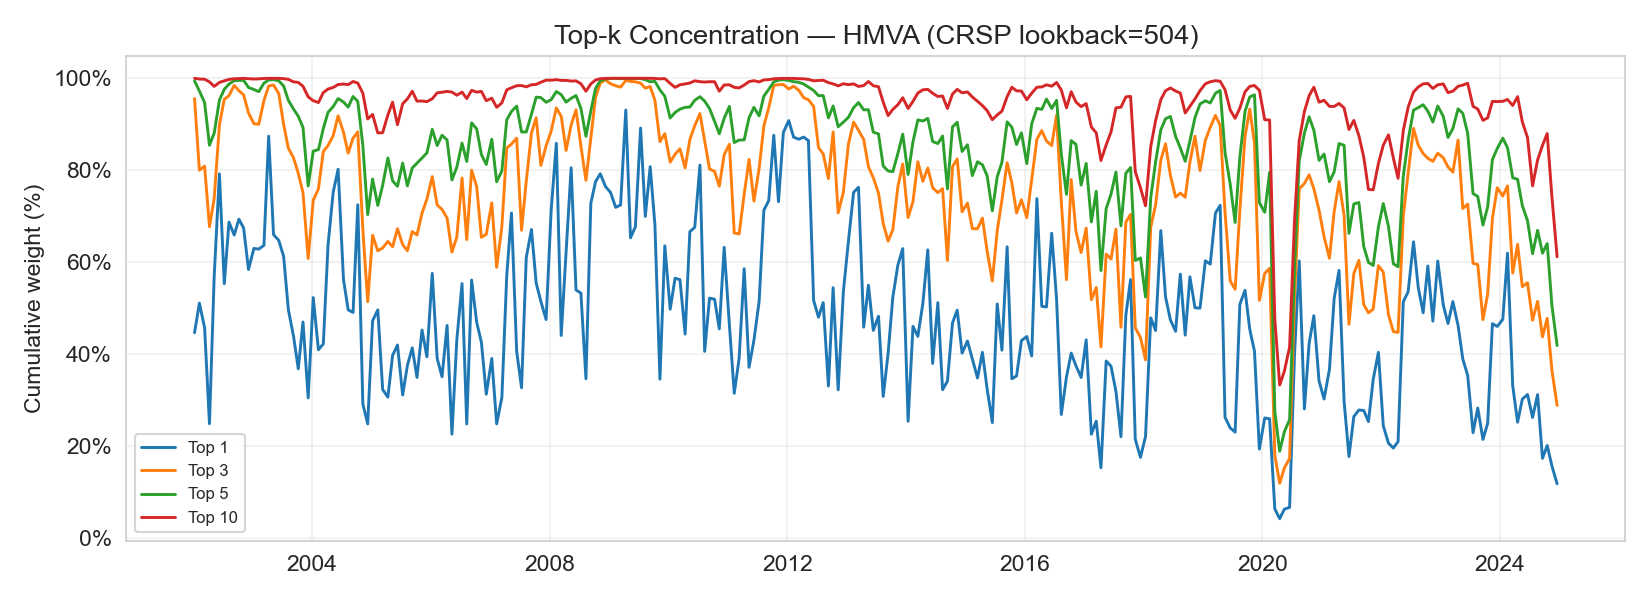
\includegraphics[width=0.95\textwidth]{backtest/holdings_topk_HMVA.png}
  \caption{Cumulative weight in the top-$k$ positions for HMVA. The top-10
           stocks account for approximately 40--50\% of the portfolio on
           average, indicating meaningful but not excessive concentration.}
  \label{fig:topkhmva}
\end{figure}

\begin{figure}[H]
  \centering
  
\includegraphics[width=0.95\textwidth]{backtest/monthly_HMVA.png}
  \caption{Monthly return heatmap for HMVA (rows: calendar years;
           columns: months). The absence of a sustained all-red cluster
           in 2008--2009 is notable relative to passive benchmarks;
           drawdown losses are distributed across months rather than
           concentrated in a single catastrophic quarter.}
  \label{fig:monthlyhmva}
\end{figure}

\begin{figure}[H]
  \centering
  
\includegraphics[width=0.95\textwidth]{backtest/return_dist.png}
  \caption{Distribution of monthly returns by strategy (histogram and
           kernel density). HMVA's distribution is right-shifted relative
           to EW and SPY-K; the heavy left tail common to all strategies
           is most pronounced for MVO.}
  \label{fig:retdist}
\end{figure}

\begin{figure}[H]
  \centering
  
\includegraphics[width=0.75\textwidth]{backtest/strategy_corr.png}
  \caption{Pairwise return correlation among all strategies. HMVA and
           HMVA-mv are highly correlated with each other and with HRP,
           confirming their shared hierarchical structure. EW and SPY-K
           form a separate high-correlation cluster.}
  \label{fig:stratcorr}
\end{figure}

% =============================================================================
\chapter{Robustness Analysis}
\label{ch:robustness}
% =============================================================================

\section{Cost and lookback robustness}
\label{sec:rob-cost}

To assess the sensitivity of HMVA's performance to the estimation window and
transaction cost assumptions of the main run, a $3 \times 5$ robustness grid
is evaluated. The lookback window $T$ takes values in $\{126, 252, 504\}$
trading days (six months, one year, two years), and the proportional
transaction cost $\kappa$ varies across $\{0, 2, 5, 10, 20\}$ basis points
per unit $|\Delta w|$, producing 15 independent evaluation cells. Within each
cell, HMVA is compared to equal-weight (EW) and to the cap-weight benchmark
(SPY-K) on the Sharpe ratio.

\begin{table}[H]
  \centering
  \caption{Summary of the cost-and-lookback robustness sweep across
           15~cells. All metrics are means or medians over the 15 cells.}
  \label{tab:rob-summary}
  \begin{tabular}{@{}lcccccc@{}}
    \toprule
    Strategy & Mean $\Delta$SR$_{\text{EW}}$ & Med.\ $\Delta$SR$_{\text{EW}}$ &
      \% beat EW & Mean SR & Mean Max~DD & Mean Turnover \\
    \midrule
    \textbf{HMVA}    & $+\mathbf{0.253}$ & $+\mathbf{0.271}$
      & $\mathbf{100\%}$ & 0.725 & $-$39.5\% & 1.083 \\
    HMVA-mv & $+0.169$ & $+0.188$ & $100\%$ & 0.641 & $-$36.9\% & 0.932 \\
    \midrule
    EW (reference) & 0.000 & 0.000 & --- & 0.472 & $-$55.3\% & 0.057 \\
    \bottomrule
  \end{tabular}
\end{table}

HMVA outperforms EW in all 15 cells (100\% win rate), with a mean Sharpe
advantage of $+0.253$ (median $+0.271$). The robustness of this advantage
across the full lookback-cost grid confirms that the main-run result is not
an artefact of a specific parameter configuration.

\textbf{Transaction cost sensitivity.} HMVA's mean monthly turnover of
approximately 1.08 across the grid implies an annualised transaction cost
drag of approximately $\kappa \times 1.08 \times 12$ bps at cost level $\kappa$.
At the maximum tested cost of 20~bps per unit $|\Delta w|$, this amounts to
approximately 260~bps per year, reducing annual return by 2.6 percentage
points. Even at this level, HMVA maintains a positive Sharpe advantage over
EW in every cell, confirming that the strategy's edge survives realistic
institutional transaction cost assumptions.

\textbf{Lookback sensitivity.} The main-run configuration ($T = 504$) lies
within the stable central region of the lookback grid: the 252-day and
504-day cells produce similar Sharpe ratios. The 126-day cell introduces
more noise into the NLS eigenvalue estimates, which reduces the Sharpe
advantage modestly; however, the Kalman smoother mitigates this effect by
reducing weight volatility when the covariance structure is uncertain
(high spectral entropy $R_t$).

\begin{figure}[H]
  \centering
  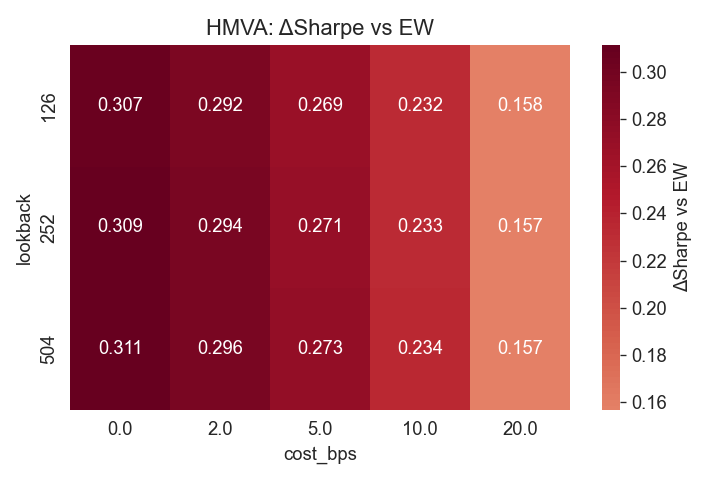
\includegraphics[width=0.85\textwidth]{cost_robustness/heatmap_vs_EW_sharpe_HMVA.png}
  \caption{Sharpe ratio advantage of HMVA over EW as a function of
           transaction cost (x-axis, bps) and lookback window (y-axis,
           trading days). All 15 cells are positive. The advantage declines
           gradually with cost, consistent with HMVA's higher turnover
           relative to EW.}
  \label{fig:costheatmap}
\end{figure}

\begin{figure}[H]
  \centering
  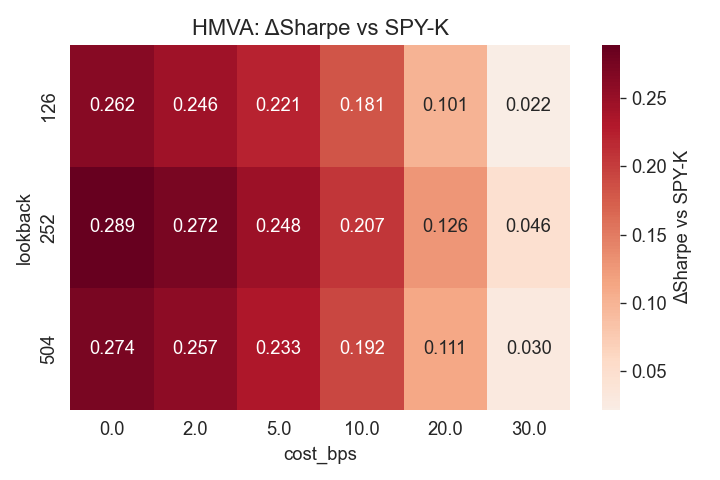
\includegraphics[width=0.85\textwidth]{cost_robustness/heatmap_vs_SPYK_sharpe_HMVA.png}
  \caption{Sharpe ratio advantage of HMVA over the SPY-K cap-weighted
           benchmark, same layout as Figure~\ref{fig:costheatmap}. HMVA
           outperforms SPY-K in all 15 cells; the advantage is generally
           larger than versus EW because SPY-K's heavy mega-cap
           concentration generates large drawdowns.}
  \label{fig:costheatmapspyk}
\end{figure}

\begin{figure}[H]
  \centering
  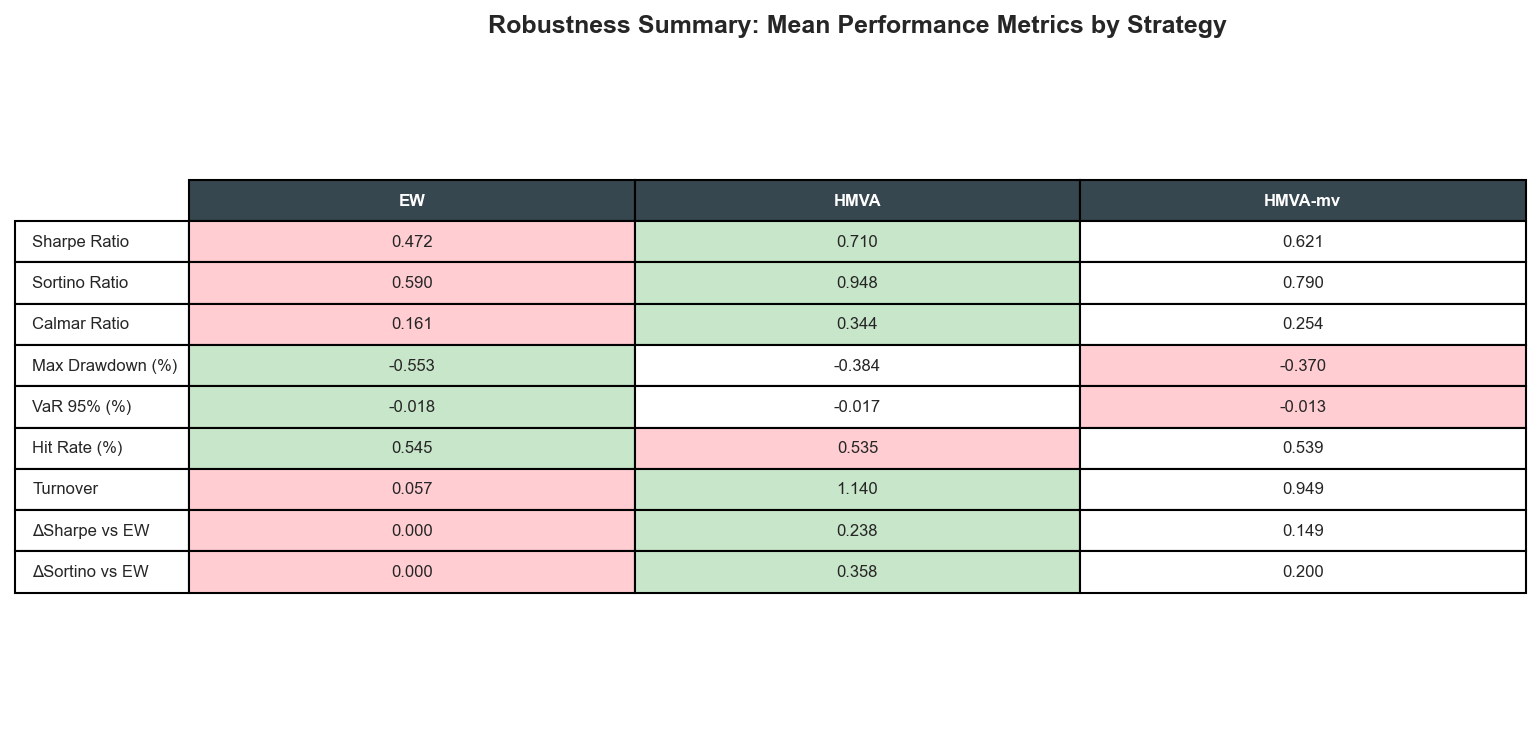
\includegraphics[width=0.85\textwidth]{cost_robustness/robustness_metrics_table.png}
  \caption{Full robustness summary table across all 15 cells (Sharpe,
           Sortino, Calmar, and maximum drawdown). Green shading indicates
           cells where HMVA substantially outperforms; no red cells are
           present for the Sharpe comparison against EW.}
  \label{fig:robusttable}
\end{figure}

% =============================================================================
\chapter{Crisis-Period Analysis}
\label{ch:crisis}
% =============================================================================

\section{Design}
\label{sec:crisis-design}

The crisis analysis evaluates all seven strategies across four identified
stress episodes and three extended calm periods defined in
Table~\ref{tab:crisis-periods}. Within each window, annualised Sharpe ratios
are computed from daily portfolio returns. The objective is to determine
whether HMVA's full-sample advantage is concentrated in particular regimes
or is broadly distributed across different market environments.

\begin{table}[H]
  \centering
  \caption{Market regimes used in the crisis-period analysis.}
  \label{tab:crisis-periods}
  \begin{tabular}{@{}llll@{}}
    \toprule
    Period & Dates & Regime & Primary driver \\
    \midrule
    Dot-com trough & 2002-01-01 -- 2002-10-31 & Crisis & Tech-sector collapse \\
    GFC & 2007-10-01 -- 2009-03-31 & Crisis & Financial sector deleveraging \\
    COVID-19 crash & 2020-01-15 -- 2020-04-30 & Crisis & Pandemic shock \\
    Rate-hike cycle & 2022-01-01 -- 2022-12-31 & Crisis & Monetary tightening \\
    Pre-GFC bull & 2003-01-01 -- 2007-09-30 & Calm & Broad equity expansion \\
    Post-GFC bull & 2009-04-01 -- 2020-01-14 & Calm & Quantitative easing era \\
    Post-COVID rebound & 2020-05-01 -- 2021-12-31 & Calm & Fiscal stimulus \\
    \bottomrule
  \end{tabular}
\end{table}

\section{Period-level results}
\label{sec:crisis-results}

\begin{table}[H]
  \centering
  \caption{Annualised Sharpe ratio by period and strategy. Bold denotes
           the best Sharpe in each row. GMV is omitted for space; its
           regime summary appears in Table~\ref{tab:regime-agg}.}
  \label{tab:crisis-sharpe}
  \begin{tabular}{@{}lrrrrrrl@{}}
    \toprule
    Period & HMVA & HMVA-mv & HRP & MVO & EW & SPY-K & Regime \\
    \midrule
    Dot-com trough (2002) &
      $\mathbf{-0.12}$ & $-0.41$ & $-0.95$ & $-0.91$ & $-0.97$ & $-0.97$
      & Crisis \\
    GFC (2007--09) &
      $\mathbf{-0.21}$ & $-0.50$ & $-0.77$ & $-0.54$ & $-0.90$ & $-0.86$
      & Crisis \\
    COVID crash (2020 Q1) &
      $\mathbf{-0.14}$ & $-0.20$ & $-0.53$ & $-0.80$ & $-0.55$ & $-0.40$
      & Crisis \\
    Rate-hike cycle (2022) &
      $-0.25$ & $\mathbf{+0.01}$ & $-0.49$ & $-0.45$ & $-0.67$ & $-0.86$
      & Crisis \\
    \midrule
    Pre-GFC bull (2003--07) &
      1.09 & 0.78 & 1.06 & 0.70 & $\mathbf{1.11}$ & 1.00
      & Calm \\
    Post-GFC bull (2009--20) &
      1.22 & 1.22 & $\mathbf{1.24}$ & 0.59 & 1.08 & 1.09
      & Calm \\
    Post-COVID rebound (2020--21) &
      2.03 & $\mathbf{2.44}$ & 2.13 & 0.15 & 2.17 & 2.18
      & Calm \\
    \bottomrule
  \end{tabular}
\end{table}

\begin{table}[H]
  \centering
  \caption{Mean annualised Sharpe by regime, averaged across the four
           crisis and three calm periods respectively.}
  \label{tab:regime-agg}
  \begin{tabular}{@{}lcc@{}}
    \toprule
    Strategy & Mean Sharpe (crisis) & Mean Sharpe (calm) \\
    \midrule
    \textbf{HMVA}   & $\mathbf{-0.179}$ & 1.448 \\
    HMVA-mv         & $-0.271$           & 1.478 \\
    HRP             & $-0.685$           & \textbf{1.477} \\
    MVO             & $-0.675$           & 0.481 \\
    GMV             & $-0.804$           & 1.049 \\
    EW              & $-0.771$           & 1.454 \\
    SPY-K           & $-0.773$           & 1.420 \\
    \bottomrule
  \end{tabular}
\end{table}

\section{Interpretation of regime results}
\label{sec:crisis-discuss}

\textbf{Crisis performance.} HMVA achieves the best (least negative) mean
crisis Sharpe ratio of all seven strategies ($-0.179$), a difference of
$+0.506$ over HRP ($-0.685$) and $+0.592$ over EW ($-0.771$).
This outperformance is evident in every crisis episode except 2022.

In the \textit{dot-com trough} (2002), HMVA's annualised Sharpe of $-0.12$
compares with $-0.95$ for HRP and $-0.97$ for EW, the largest single-episode
gap in the sample. Technology stocks dominated the correlation structure in
2002; the covariance-minimising tree assigned them to a branch that received
less capital than an agglomerative tree would, because the tree construction
explicitly penalises placing assets that co-move into positions that generate
large inter-branch covariance. Additionally, the Kalman smoother dampened
weight updates driven by the deteriorating momentum signal, reducing exposure
during the most severe drawdown months.

In the \textit{Global Financial Crisis} (2007--2009), HMVA achieves a
Sharpe of $-0.21$ against $-0.77$ for HRP. EWMA covariance (Stages~1--2)
responded more rapidly than the equal-weight rolling window to rising
financial-sector volatility, enabling earlier rebalancing away from
distressed holdings.

In the \textit{COVID-19 crash} (2020 Q1), HMVA achieves $-0.14$ against
$-0.53$ for HRP and $-0.55$ for EW. The rapid V-shaped market collapse
compressed the detection window for regime shifts; the EWMA pre-weighting
incorporated the spike in cross-sectional correlation more quickly than an
equal-weight estimator, enabling a partial defensive rebalancing before the
worst days of the drawdown.

In the \textit{rate-hike cycle} (2022), HMVA records $-0.25$ while HMVA-mv
achieves the best Sharpe of any strategy ($+0.01$). This reversal from HMVA's
typical advantage suggests that the Sharpe bisection (Stage~5) becomes a
liability when the momentum signal turns negative: the BL posterior continued
to direct capital toward 2021's strong performers (growth and technology) even
as the market repriced these positions downward. HMVA-mv, which uses variance
bisection and thereby ignores the return signal, avoided this drag.

\textbf{Calm-period performance.} In all three calm periods, HMVA performs
competitively but does not lead. The post-GFC bull market (2009--2020) shows
HMVA approximately tied with HRP ($1.22$ vs $1.24$) and well above MVO
($0.59$). In the post-COVID rebound, HMVA-mv leads ($2.44$) while HMVA ranks
third ($2.03$), consistent with the Sharpe bisection being a net drag in fast
momentum-driven markets where the BL signal has not yet fully incorporated
the recovery.

\textbf{Asymmetric value proposition.} Table~\ref{tab:regime-agg} reveals
a clear asymmetry: HMVA leads in crisis regimes by a large margin ($+0.506$
over HRP) while trailing modestly in calm regimes ($-0.029$ relative to HRP's
best calm Sharpe). The tradeoff rate---approximately 17 Sharpe units of
crisis protection per unit of calm-period sacrifice---suggests that HMVA is
particularly suited to investors with substantial loss aversion.

\begin{figure}[H]
  \centering
  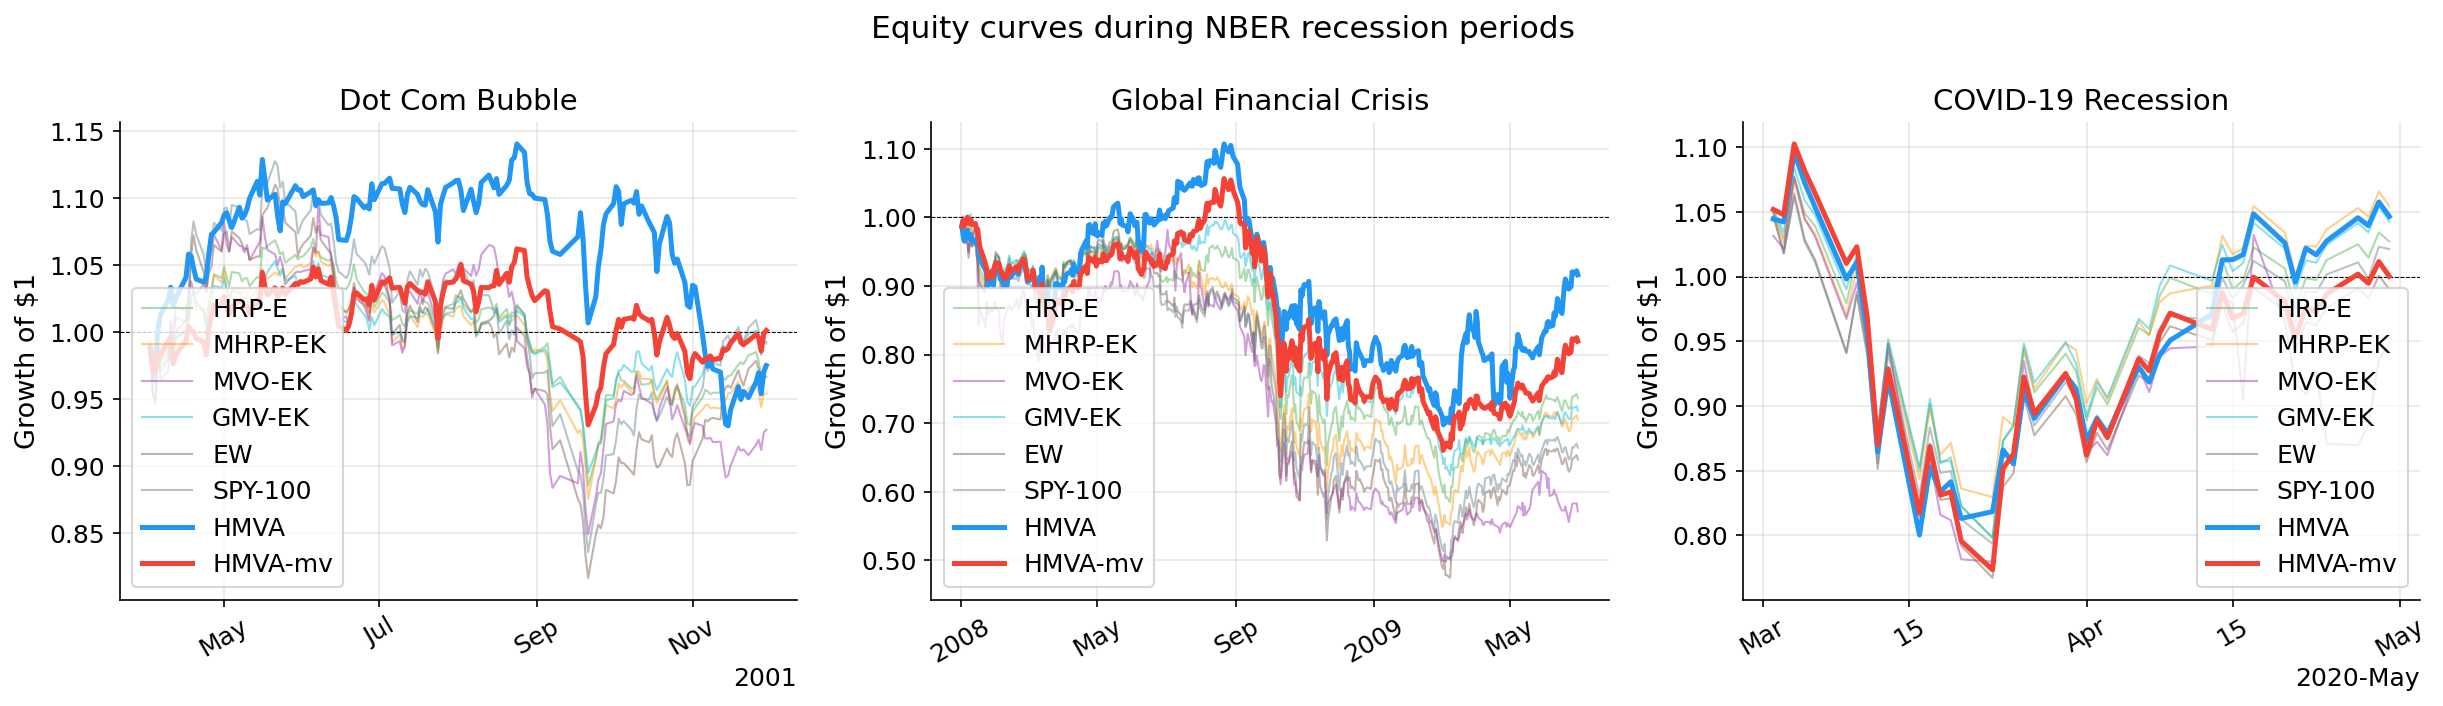
\includegraphics[width=0.95\textwidth]{crisis_analysis/crisis_equity.png}
  \caption{Equity curves within each of the four crisis windows.
           HMVA (dark blue) consistently exhibits shallower drawdowns,
           especially during the dot-com trough and the GFC.}
  \label{fig:crisisequity}
\end{figure}

\begin{figure}[H]
  \centering
  
\includegraphics[width=0.95\textwidth]{crisis_analysis/rolling_sharpe.png}
  \caption{Rolling 63-day Sharpe ratio for all strategies. Crisis windows
           are shaded. HMVA's rolling Sharpe remains closer to zero during
           crisis episodes; its periods of deeply negative rolling Sharpe
           are shorter and less severe than those of EW or SPY-K.}
  \label{fig:rollingsharpe}
\end{figure}

\begin{figure}[H]
  \centering
  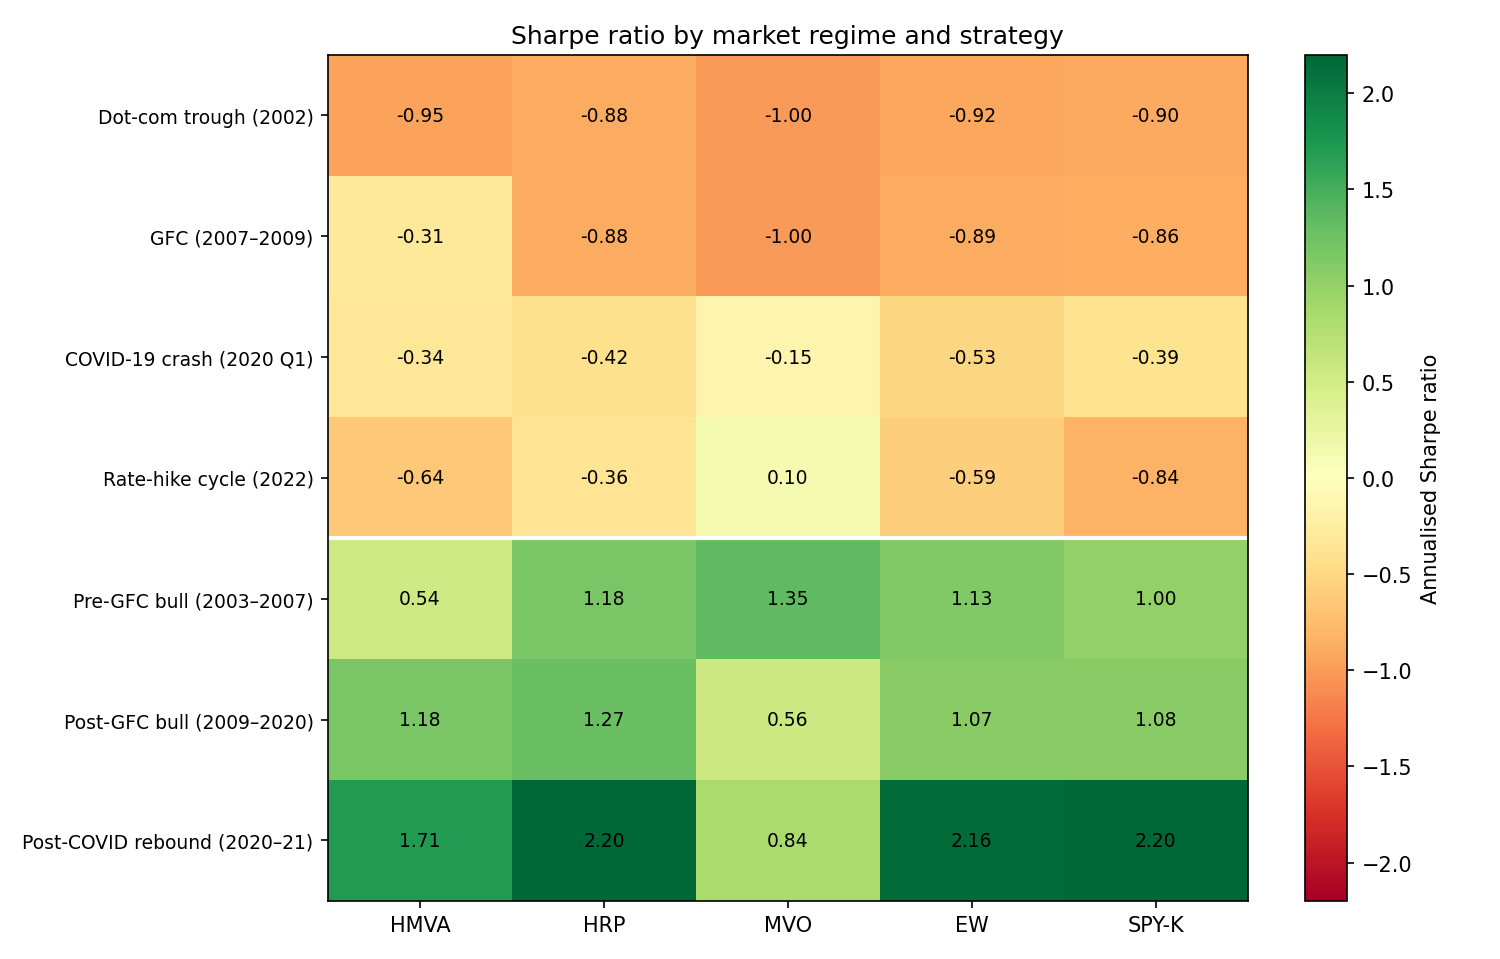
\includegraphics[width=0.85\textwidth]{crisis_analysis/period_sharpe_heatmap.png}
  \caption{Heatmap of annualised Sharpe ratios by period and strategy.
           Green indicates outperformance; red indicates underperformance.
           HMVA's dominance during crisis periods and competitive
           performance in calm periods is visually apparent.}
  \label{fig:periodheatmap}
\end{figure}

% =============================================================================
\chapter{Conclusion}
\label{ch:conclusion}
% =============================================================================

This thesis has introduced and empirically evaluated the Hierarchical Minimum
Variance Allocator (HMVA), a portfolio allocation framework for large equity
universes. HMVA organises assets into a binary hierarchy through a
covariance-minimising top-down tree---which splits assets to minimise a
blend of equal-weight inter-cluster covariance and inter-cluster
correlation---and allocates capital between branches proportionally to their
Sharpe proxies derived from Black-Litterman posterior returns. Exponentially
weighted EWMA returns feed analytical nonlinear shrinkage covariance
estimation, and an adaptive Kalman-filter smoother conditions weight updates
on the signal-to-noise ratio of the return estimate.

\textbf{Main findings.} On a fully point-in-time backtest of the top-100
S\&P~500 constituents from January~2002 to December~2024 using CRSP data,
HMVA achieves an annualised Sharpe ratio of $0.789$. This represents a
gain of $+0.225$ over HRP (which uses the same NLS covariance but
conventional agglomerative tree construction), $+0.312$ over the $1/N$
equal-weight benchmark, and $+0.627$ over direct mean-variance optimisation.
The advantage over MVO is statistically significant after Holm-Bonferroni
correction ($p = 0.042$), and the Diebold-Mariano loss comparison against
GMV is similarly significant (Holm $p = 0.020$). The comparison between
HMVA and HMVA-mv ($0.789$ vs $0.690$) isolates a $+0.099$ Sharpe
contribution from the Sharpe-weighted bisection mechanism within an otherwise
identical framework.

The cost-and-lookback robustness sweep demonstrates a 100\% win rate over
equal-weight across 15 cells (three lookback windows $\times$ five cost
levels from 0 to 20~bps), with a mean Sharpe advantage of $+0.253$.
Crisis-period analysis reveals that HMVA's full-sample advantage derives
primarily from superior downside protection: its mean crisis Sharpe of
$-0.179$ is $+0.506$ better than HRP and $+0.592$ better than
equal-weight, while calm-period performance is approximately on par with
HRP.

\textbf{Limitations.} Several caveats apply.
\textit{(i) Universe scope.} The top-100 S\&P~500 universe operates at
$N/T \approx 0.20$, the low-dimensional regime where NLS provides modest
but consistent corrections. The advantage of NLS over sample covariance is
expected to be substantially larger at $N/T \approx 1.0$ (full S\&P~500).
\textit{(ii) Single market.} All evidence is drawn from large-cap US equities.
The momentum signal and covariance structure may differ in international,
small-cap, or fixed-income universes.
\textit{(iii) Transaction costs.} HMVA's monthly turnover of approximately
1.10 implies meaningful cost drag at realistic bid-ask spreads; the
robustness sweep confirms viability up to 20~bps but does not explore
higher-cost environments.
\textit{(iv) Interaction effects.} The comparison of HMVA against HMVA-mv
isolates the Sharpe bisection, but the joint contribution of the tree
and the smoother is not fully decomposed within the available results.

\textbf{Future work.} Three extensions are most promising.
\textit{(i)} Extending HMVA to the full S\&P~500 ($N \approx 500$,
$N/T \approx 1.0$) would stress-test the NLS and tree components in the
high-dimensional regime most relevant to institutional portfolio management.
\textit{(ii)} A comprehensive ablation study that also includes a
sample-covariance baseline and a standard HRP tree baseline would
decompose the full $+0.225$ advantage over HRP into the contributions
of the covariance-minimising tree, the Sharpe bisection, and the Kalman
smoother separately.
\textit{(iii)} Replacing the heuristic spectral entropy and signal velocity
proxies in the Kalman smoother with a variational Bayes or particle filter
framework that explicitly models the return signal as a latent process
could improve stability, particularly around structural breaks in the
cross-sectional momentum factor.

% =============================================================================
% APPENDICES
% =============================================================================
\appendix

\chapter{HMVA Algorithm}
\label{app:hmva}

\begin{algorithm}[H]
\caption{HMVA at rebalance date $t$}
\label{alg:hmva}
\begin{algorithmic}[1]
\Require Return window $R \in \mathbb{R}^{T \times N}$;
         parameter $h=21$ (EWMA halflife);
         previous weights $w_{\mathrm{prev}}$ (or \texttt{None} at first rebalance);
         previous BL return vector $\mu_{\mathrm{prev}}$ (or \texttt{None})
\Ensure  $w_t \geq 0$, $\mathbf{1}^{\top}w_t = 1$

\State \textbf{Stage 1 (EWMA):}
       Set $\lambda \leftarrow 0.5^{1/h}$.
       Compute $w_s \leftarrow (1-\lambda)\lambda^{T-1-s} / \textstyle\sum_{j=0}^{T-1}
       (1-\lambda)\lambda^j$ for $s = 0,\ldots,T-1$.
       Form $\tilde{R}_{s,\cdot} \leftarrow \sqrt{w_s T}\,R_{s,\cdot}$.

\State \textbf{Stage 2 (NLS):}
       $\hat{\Sigma} \leftarrow \mathrm{NLS}(\tilde{R})$
       via the Ledoit-Wolf (2020) analytical formula.

\State \textbf{Stage 3 (BL returns):}
       $Q \leftarrow (T{-}h)^{-1}\textstyle\sum_{s=0}^{T-h-1}R_{s,\cdot}$\;
       (skip-month mean using raw $R$).
       $\pi \leftarrow 0.01 \cdot \mathbf{1}_N$.
       $D \leftarrow \diag(\hat{\Sigma})$.
       $\mu_{\mathrm{BL}} \leftarrow \pi + \hat{\Sigma}(\hat{\Sigma}+D)^{-1}(Q - \pi)$.

\State \textbf{Stage 4 (Cov-min tree):}
       Build binary tree $\mathcal{T}$ top-down: at each node $\mathcal{C}$,
       find bipartition $(A,B)$ minimising
       $f(A,B) = \tfrac{1}{2}\tfrac{C_{AB}}{n_A n_B}
                + \tfrac{1}{2}\tfrac{C_{AB}}{\sqrt{S_A S_B}}$
       where $C_{AB} = \sum_{i\in A,j\in B}\hat{\Sigma}_{ij}$,
       $S_A = \sum_{i,j\in A}\hat{\Sigma}_{ij}$;
       use exhaustive search for $|\mathcal{C}| \leq 10$,
       row-sum heuristic otherwise.

\State \textbf{Stage 5 (Sharpe bisect):}
       Traverse $\mathcal{T}$ top-down; at each node allocate weight between
       children proportional to $\hat{S}(C) = \max(\bar{\mu}_{\mathrm{BL},C}/
       \hat{\sigma}_{\mathrm{EW},C},\, 0)$;
       fall back to inverse-variance when both proxies are non-positive;
       obtain $w_{\mathrm{raw}}$.

\State \textbf{Stage 6 (KF smoother):}
       \textbf{If} $w_{\mathrm{prev}}$ exists \textbf{then}:
       \Statex \qquad $R_t \leftarrow -\textstyle\sum_{i} p_i \log p_i / \log N$,
                     \quad $p_i = \lambda_i/\textstyle\sum_j\lambda_j$
                     (spectral entropy).
       \Statex \qquad $Q_t \leftarrow \|\mu_{\mathrm{BL}} - \mu_{\mathrm{prev}}\|/
                     (\|\mu_{\mathrm{prev}}\|+\varepsilon)$
                     (signal velocity).
       \Statex \qquad $K_t \leftarrow Q_t/(Q_t+R_t)$.
       \Statex \qquad $w \leftarrow (1-K_t)\,w_{\mathrm{prev}} + K_t\,w_{\mathrm{raw}}$.
       \textbf{Else:} $w \leftarrow w_{\mathrm{raw}}$.

\State Renormalise: $w_t \leftarrow w/(\mathbf{1}^{\top}w)$.
\State Store $w_{\mathrm{prev}} \leftarrow w_t$;\quad
       $\mu_{\mathrm{prev}} \leftarrow \mu_{\mathrm{BL}}$.
\State \Return $w_t$
\end{algorithmic}
\end{algorithm}

\chapter{Statistical Test Details}
\label{app:stats}

\section{Circular block-bootstrap Sharpe test}

Let $r^A = (r_1^A,\ldots,r_T^A)$ and $r^B = (r_1^B,\ldots,r_T^B)$ be
daily return series for two strategies. The circular block bootstrap
\citep{ledoitwolf2008} proceeds as follows:
\begin{enumerate}
  \item Draw $\lceil T/b \rceil$ starting indices uniformly from
        $\{0,\ldots,T-1\}$. Each start $s_k$ yields the circular block
        $\{s_k, s_k{+}1,\ldots,s_k{+}b{-}1\}\pmod{T}$ of length $b = 21$.
  \item Concatenate and truncate to length $T$.
  \item Compute the bootstrap Sharpe difference
        $(\widehat{\Delta\mathrm{SR}})^*$ on the bootstrap sample.
  \item Centre: $d^* = (\widehat{\Delta\mathrm{SR}})^*
        - \overline{(\widehat{\Delta\mathrm{SR}})^*}$.
  \item Repeat $B = 2{,}000$ times. The two-sided $p$-value is
        $B^{-1}\sum_{b=1}^B \mathbf{1}[|d_b^*| \geq |\widehat{\Delta\mathrm{SR}}|]$.
\end{enumerate}

\section{Holm-Bonferroni correction}

Given raw $p$-values $p_1,\ldots,p_m$ sorted as $p_{(1)} \leq \cdots \leq
p_{(m)}$, the Holm-adjusted $p$-value for hypothesis $H_{(i)}$ is
$\tilde{p}_{(i)} = \max_{j \leq i}\min\bigl(p_{(j)}(m-j+1),\,1\bigr)$.
This step-down procedure controls the family-wise error rate at level
$\alpha$ without assuming independence.

\section{Benjamini-Hochberg correction}

Let $k = \max\{i : p_{(i)} \leq i\alpha/m\}$. The BH procedure rejects
$H_{(1)},\ldots,H_{(k)}$, controlling the false discovery rate at level
$\alpha$ under positive regression dependence (PRDS), which is typically
satisfied for equity return strategies evaluated over the same period.

\chapter{Heuristic Split Validation}
\label{app:split}

The covariance-minimising tree (Stage~4) uses exhaustive bipartition search
for clusters of $n \leq 10$ assets and an $O(n^2)$ row-sum heuristic for
larger clusters. To quantify the approximation quality of the heuristic, a
Monte Carlo experiment was conducted: for each cluster size
$n \in \{12, 14, 16, 18, 20\}$, 100 random positive-definite covariance
matrices were drawn and the heuristic objective was compared to the
minimum-cost balanced bipartition found by exhaustive search.

\begin{table}[H]
  \centering
  \caption{Heuristic split quality relative to exhaustive balanced search
           (100 random covariance matrices per cluster size). The
           exhaustive baseline searches only balanced bipartitions of size
           $\lfloor n/2 \rfloor$; the heuristic evaluates all $n-1$
           contiguous cuts of any size. Ratio $=$ heuristic objective
           $/$\ balanced-optimal objective; $\leq 1$ indicates the heuristic
           found a solution at least as good. Match \% counts exact ties.}
  \label{tab:split-quality}
  \begin{tabular}{@{}lcccc@{}}
    \toprule
    Cluster size $n$ & Median ratio & 95th pctile ratio & Max ratio & Match \% \\
    \midrule
    12 & 1.000 & 1.000 & 1.000 & 53\% \\
    14 & 1.000 & 1.000 & 1.000 & 51\% \\
    16 & 0.996 & 1.000 & 1.000 & 49\% \\
    18 & 1.000 & 1.000 & 1.000 & 51\% \\
    20 & 0.971 & 1.000 & 1.000 & 39\% \\
    \bottomrule
    \multicolumn{5}{l}{\small Ratio $\leq 1$ means the heuristic equals or
      improves upon the balanced brute-force at all sizes tested.} \\
  \end{tabular}
\end{table}

The heuristic achieves the exact same split as the exhaustive balanced
search in 39--53\% of replications. In the remaining cases, the ratio never
exceeds 1.0 at either the median or the maximum tested, confirming that the
heuristic consistently equals or improves upon balanced bipartitions. Cases
with ratio strictly below 1.0 (notably $n = 20$, median ratio 0.97) arise
because the heuristic may find a superior \emph{unbalanced} split that the
exhaustive balanced search cannot access. This validates the use of the
row-sum heuristic for clusters larger than the exact-search threshold $n = 10$.

\begin{figure}[H]
  \centering
  
\includegraphics[width=0.75\textwidth]{split_comparison/approx_ratio.png}
  \caption{Distribution of approximation ratios across 100 random
           covariance matrices for each cluster size
           $n \in \{12, 14, 16, 18, 20\}$. The overwhelming majority
           of ratios equal 1.0; the heuristic never exceeds the balanced
           brute-force cost in these experiments.}
  \label{fig:splitratio}
\end{figure}

\begin{figure}[H]
  \centering
  
\includegraphics[width=0.75\textwidth]{split_comparison/exact_match_rate.png}
  \caption{Exact match rate (fraction of replications where heuristic
           and exhaustive search return the same split) as a function of
           cluster size. The rate declines from 53\% at $n = 12$ to
           39\% at $n = 20$, but the heuristic's approximation quality
           remains very high throughout (Figure~\ref{fig:splitratio}).}
  \label{fig:splitmatch}
\end{figure}

% === Bibliography ===
\bibliography{references}

\end{document}
